\documentclass[border=1pt]{standalone}
\usepackage{fontspec}
\setmainfont{CMU Sans Serif}
\setsansfont{CMU Sans Serif}
\usepackage{tikz}
\usetikzlibrary{arrows.meta, positioning}
\usepackage{amsmath}
\usepackage{xcolor}

\definecolor{Purple}{RGB}{113, 80, 224}

\begin{document}
\resizebox{3in}{!}{%
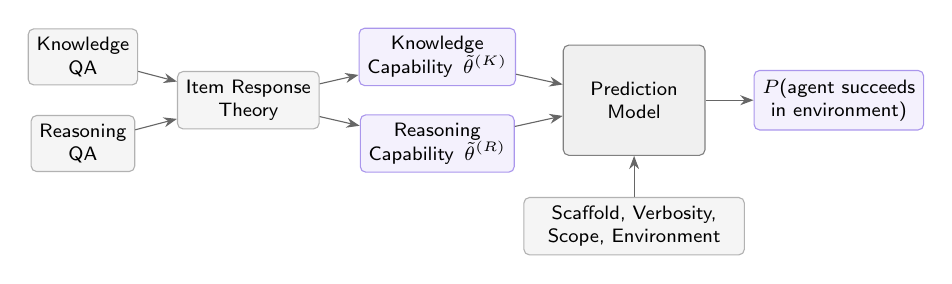
\begin{tikzpicture}[
    >=Stealth,
    box/.style={
        draw=black!30, rounded corners=2pt, fill=white,
        minimum height=0.55cm, align=center,
        font=\footnotesize\sffamily, inner sep=3pt
    },
    purplebox/.style={
        draw=Purple!60, fill=Purple!8, rounded corners=2pt,
        minimum height=0.55cm, align=center,
        font=\footnotesize\sffamily, inner sep=3pt
    },
    blackbox/.style={
        draw=black!50, rounded corners=2pt, fill=black!6,
        minimum height=1.4cm, minimum width=1.8cm, align=center,
        font=\footnotesize\sffamily, inner sep=4pt
    },
    arr/.style={-Stealth, thin, black!60},
]

%% QA inputs
\node[box, fill=gray!8] (kqa) at (0, 0.55)
    {\scriptsize Knowledge\\[-1pt]\scriptsize QA};
\node[box, fill=gray!8] (rqa) at (0, -0.55)
    {\scriptsize Reasoning\\[-1pt]\scriptsize QA};

%% Item Response Theory
\node[box, fill=gray!8] (irt) at (2.1, 0)
    {\scriptsize Item Response\\[-1pt]\scriptsize Theory};

\draw[arr] (kqa) -- (irt);
\draw[arr] (rqa) -- (irt);

%% Capabilities
\node[purplebox] (capk) at (4.5, 0.55)
    {\scriptsize Knowledge\\[-1pt]\scriptsize Capability\, $\tilde{\theta}^{\scriptscriptstyle(K)}$};
\node[purplebox] (capr) at (4.5, -0.55)
    {\scriptsize Reasoning\\[-1pt]\scriptsize Capability\, $\tilde{\theta}^{\scriptscriptstyle(R)}$};

\draw[arr] (irt) -- (capk);
\draw[arr] (irt) -- (capr);

%% Prediction model
\node[blackbox] (pred) at (7.0, 0)
    {\scriptsize Prediction\\[-1pt]\scriptsize Model};

\draw[arr] (capk) -- (pred);
\draw[arr] (capr) -- (pred);

%% Covariates
\node[box, fill=gray!8, minimum width=2.8cm] (covs) at (7.0, -1.6)
    {\scriptsize Scaffold, Verbosity,\\[-1pt]\scriptsize Scope, Environment};

\draw[arr] (covs.north) -- (pred.south);

%% Output
\node[purplebox] (out) at (9.6, 0)
    {\scriptsize $P$(agent succeeds\\[-1pt]\scriptsize in environment)};

\draw[arr] (pred) -- (out);

\end{tikzpicture}%
}
\end{document}
